\documentclass[14pt,final]{beamer}
%\usepackage[orientation=portrait,size=a2,scale=1.0]{beamerposter}   % e.g. for DIN-A2
\usepackage[orientation=landscape,size=a2,scale=1.0]{beamerposter}   % e.g. for DIN-A2 
  
\usetheme{winslabposter}



\title{WINS Lab Poster Template}
\author{List of authors as it appears on paper}
\footer{Contact Person: Name Surname and Email Address}
\date{\today}


\begin{document}
\begin{frame}{} 

\begin{textblock}{19.5}(1,5)
\begin{block}{About the lab\cite{einstein} } Established on the April Fools’ Day of 2016, WINS lab strives to conduct research in the field of computer networks, wireless networks, mobile systems and security thereof. We aim at building efficient and dependable solutions for the networks of the future and focus on the design and experimentation of systems and protocols. We support education both at undergraduate and graduate levels. The specific topics we study are
\begin{itemize}
\item     5G and Next Generation Mobile Networks,
\item    Internet of Things (IoT), Wireless Sensor Networks,
\item    Software Networks and Software-defined Networked Systems,
\item    Virtual Networks, Edge and Fog Computing,
\item    Cybersecurity and Network Security,
\item    Mobile Computing,
\item    Ubiquitous and Pervasive Computing, and
\item    Performance Evaluation of Networks.
\end{itemize}

\end{block}

\begin{block}{Some interesting specimens}
Stuff and nonsense
\begin{itemize}
\item 1
\begin{itemize}
\item 11
\item 12
\end{itemize}
\item $( a ), [ b ], \{ c \}, | d |, \| e \|,
\langle f \rangle, \lfloor g \rfloor,
\lceil h \rceil, \ulcorner i \urcorner$ \cite{knuthwebsite}
\end{itemize}

\end{block}
\end{textblock}

\begin{textblock}{19.3}(21.8,5)
\begin{block}{My latest paper about frogs}
Published in the \emph{Journal of Irreproducible Results}.
$$
\frac{n!}{k!(n-k)!} = \binom{n}{k}
$$
\end{block}

\begin{block}{Yet another block in the same textblock}
\begin{enumerate}
\item 1 \cite{latexcompanion}
\begin{enumerate}
\item 11
\item 12
\end{enumerate}
\item $( a ), [ b ], \{ c \}, | d |, \| e \|,
\langle f \rangle, \lfloor g \rfloor,
\lceil h \rceil, \ulcorner i \urcorner$
\end{enumerate}
\end{block}

\end{textblock}



\begin{textblock}{16.6}(42,5)
\begin{block}{A Figure}
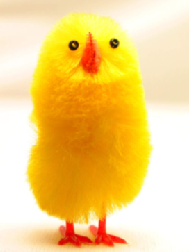
\includegraphics[width=\textwidth]{figures/Chick1.png}
\begin{equation}
A_{m,n} = 
 \begin{pmatrix}
  a_{1,1} & a_{1,2} & \cdots & a_{1,n} \\
  a_{2,1} & a_{2,2} & \cdots & a_{2,n} \\
  \vdots  & \vdots  & \ddots & \vdots  \\
  a_{m,1} & a_{m,2} & \cdots & a_{m,n} 
 \end{pmatrix}
\end{equation}

\end{block}
\end{textblock}



\begin{textblock}{30}(21.8,30)
\begin{block}{References}
\tiny
\bibliographystyle{IEEEtran}
\bibliography{refs}
\end{block}
\end{textblock}


\end{frame}
\end{document}
